\documentclass{../pl-slide}

\usepackage[british]{babel}
\usepackage[british]{datetime2}
\usepackage{ulem}
\usepackage{qrcode}

\usepackage{tikz,calc}
\usetikzlibrary{shapes, shapes, arrows, chains, fit, quotes}

\tikzstyle{trienode} = [draw=text-color, rounded corners]
\tikzstyle{bucket} = [draw=text-color, rectangle]


\settheme{ipfs-thing-2023}

%Information to be included in the title page:
\title{Reprovide Sweep}
\subtitle{Opening the DHT to large content providers}
\author{Gui Michel}
\avatar{../resources/avatar.jpg}
\handle{@guissou}
\group{Probelab}
\institute{Protocol Labs}
\event{IPFS Thing}
\date{\DTMdate{2023-04-16}}

\begin{document}

\frame{\titlepage}

\begin{frame}
\frametitle{DHT Provide Process}
When a node wants to advertise to the DHT that it provides \texttt{CID}
\bigskip
\begin{itemize}
        \itemc DHT lookup to find the \texttt{repl} (\texttt{20}) closest peers
        \begin{itemize}
        		\item[\greencube] Number of hops: $\sim 3$
        		\item[\greencube] Number of inflight messages: $\sim 10$
        		\item[\greencube] Total number of sent messages: $\sim 30$
        \end{itemize}
        \bigskip
tes        \itemc Allocate the Provider Record to these \texttt{repl} closest peers

\end{itemize}
\end{frame}

\begin{frame}
\frametitle{DHT Provide Process}

\begin{itemize}
        \itemc Number of connections opened per provide: $\sim 35$
        \begin{itemize}
        		\item[\greencube] Assume that we already have an open connection for peers in the first hop
        		\item[\greencube] Intermediary lookup peers: $\sim 15$
        		\item[\greencube] \texttt{repl} closest peers: $20$
        \end{itemize}
        \bigskip
        \itemc Number of messages sent per provide: $\sim 70$
         \begin{itemize}
        		\item[\greencube] DHT Lookup: $\sim 30 + 20$
        		\item[\greencube] Provide messages: $20$
        \end{itemize}

\end{itemize}
\end{frame}


\begin{frame}
\frametitle{Large Content Providers}

Large content provider reproviding 1 Billion CIDs every \texttt{ReprovideInterval} (22h)
\bigskip
\begin{itemize}
	\itemc Number of opened connections: $\sim 35B \approx 450'000/s$ 
	\itemc Number of messages sent: $\sim 70B \approx 900'000/s$
\end{itemize}
\end{frame}

\begin{frame}
\frametitle{Optimizing the \texttt{Reprovide} operation}

\begin{columns}[onlytextwidth]
	\begin{column}{0.69\textwidth}
		\begin{itemize}
			\itemc More CIDs to reprovide than DHT Servers
			\itemc $\Rightarrow $ multiple CIDs are allocated on the same DHT Server
			\itemc Group CIDs allocated on the same DHT Server and reprovide them sequentially
			\itemc Periodically sweep the keyspace and reprovide CIDs
			\vspace{2em}
			\item[\greencube] Minimizing the number of connections to open and messages to send
			\item[\greencube] Number of connections to open $\approx$ number of DHT server peers
		\end{itemize}
	\end{column}
	\begin{column}{0.29\textwidth}
    		\begin{center}
        		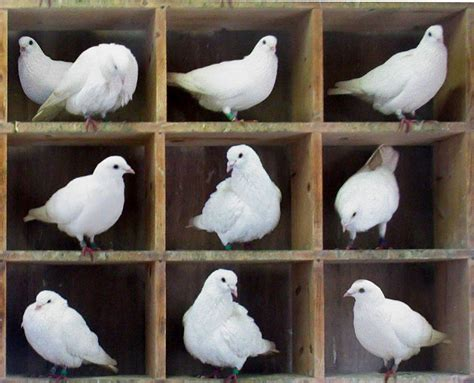
\includegraphics[width=10em]{resources/pigeonhole.jpg}
    		\end{center}
	\end{column}
\end{columns}
\end{frame}

\iffalse
\begin{frame}
	\vfill
	\begin{center}
		{\Huge Where are the binary tries?}
	\end{center}
	\vfill
\end{frame}
\fi

\begin{frame}
\frametitle{Binary Trie}

\begin{columns}[onlytextwidth]
	\begin{column}{0.39\textwidth}
		\begin{itemize}
			\itemc Binary Prefix Tree
			\itemc Data structure optimized for working with XOR distance
			\itemc Helps visualize locality in the Kademlia keyspace
			\itemc We will use them to group \textit{close} CIDs
		\end{itemize}
	\end{column}
	\begin{column}{0.59\textwidth}
    		\begin{center}
        		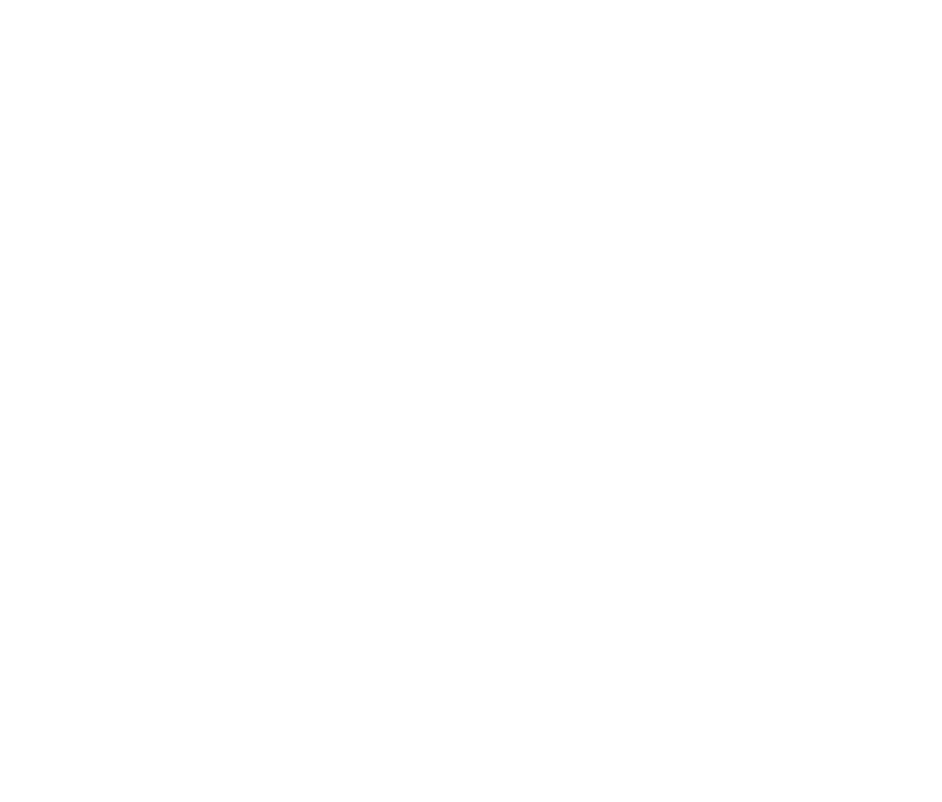
\includegraphics[height=17em]{resources/trie-compressed.png}
    		\end{center}
	\end{column}
\end{columns}

\end{frame}

\begin{frame}
\frametitle{Keyspace Regions}

\begin{columns}[onlytextwidth]
	\begin{column}{0.39\textwidth}
		\begin{itemize}
			\itemc A \texttt{Region} is defined as a prefix of the \textbf{peers} binary trie that has at least \texttt{repl} leaves.
			\itemc We are interested in the smallest possible regions fully covering the keyspace
		\end{itemize}
	\end{column}
	\begin{column}{0.59\textwidth}
    		\begin{center}
        		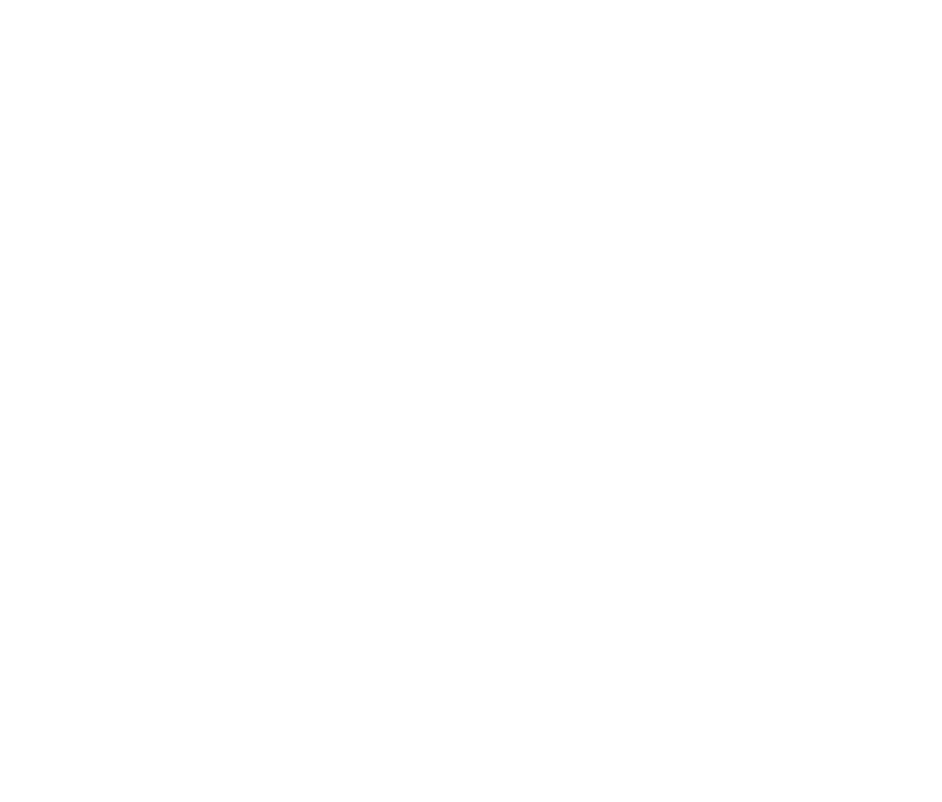
\includegraphics[height=17em]{resources/trie-compressed.png}
    		\end{center}
	\end{column}
\end{columns}

\end{frame}

\begin{frame}
\frametitle{Keyspace Regions: Example}


\begin{columns}[onlytextwidth]
	\begin{column}{0.39\textwidth}
		{\large Example: \texttt{repl = 3}}
		\bigskip
		\begin{itemize}
			\itemc Keys represent peers
			\itemc A \texttt{CID} is only stored in the region matching its prefix.
		\end{itemize}
	\end{column}
	\begin{column}{0.59\textwidth}
    		\begin{center}
        		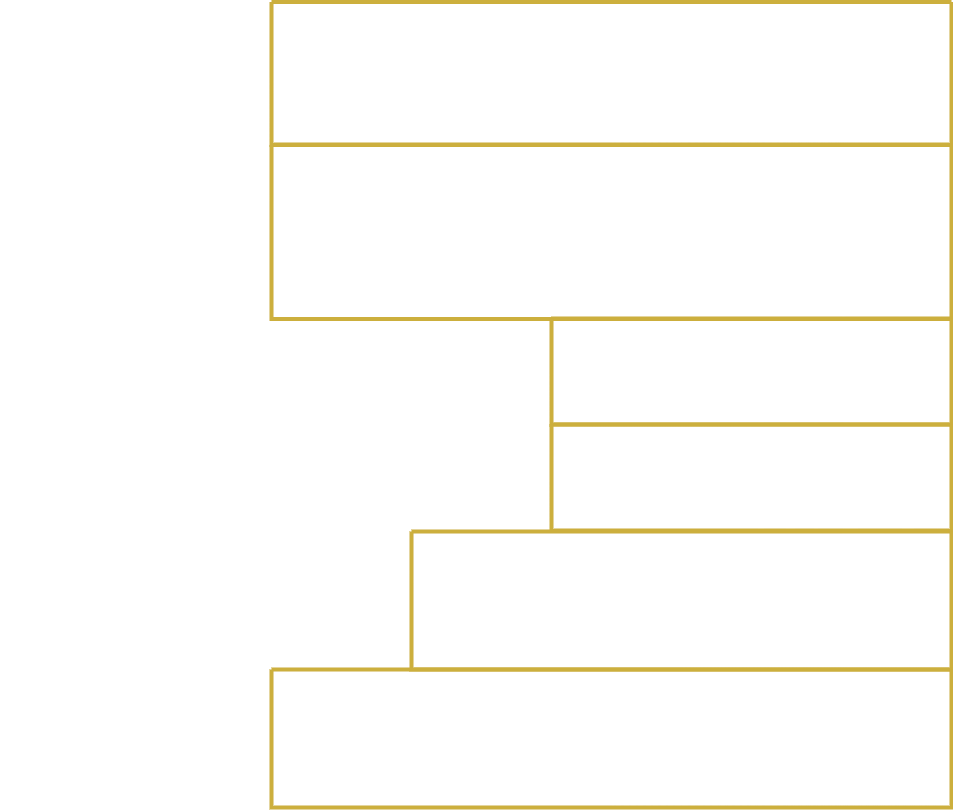
\includegraphics[height=17em]{resources/regions-defined.png}
    		\end{center}
	\end{column}
\end{columns}

\end{frame}

\begin{frame}
\frametitle{\texttt{Region} exploration}

\begin{itemize}
	\itemc Lookup a random key within the target \texttt{Region}
	\itemc If some returned peers don't match the \texttt{Region}'s prefix, \texttt{Region} is fully explored
	\itemc Else, take the largest fully explored subregion, and explore its neighbor subregion
	\itemc Repeat until the \texttt{Region} is fully explored
\end{itemize}
\end{frame}


\begin{frame}
\frametitle{Sweep}

\begin{itemize}
	\itemc Explore Kademlia keyspace \texttt{Regions} to sweep the keyspace \textit{from left to right}
	\itemc All Provider Records belonging to the looked up \texttt{Region} are reprovided
	\itemc The keyspace sweep takes \texttt{ReprovideInterval} to complete
	\bigskip
	\itemc Peers are stored in a binary trie, in order to define the \texttt{Regions}
	\itemc CIDs are stored in a distinct binary trie, for fast sweep, insert and delete
\end{itemize}
\end{frame}

\begin{frame}
\frametitle{Reproviding for a \texttt{Region}}

\begin{itemize}
	\itemc Define a temp key-value store \texttt{PeerID} $\xrightarrow{}$ \texttt{[Keys]} for \texttt{PeerID}s within the \texttt{Region}
	\itemc For all keys \texttt{k} belonging to a \texttt{Region}, add \texttt{k} to its \texttt{repl} closest peers
	\itemc Iterate over all \texttt{PeerID}s within the \texttt{Region} and reprovide all associated keys
	\itemc The number of workers can easily be limited
\end{itemize}
\end{frame}

\begin{frame}
\frametitle{\texttt{Region} Reprovide Scheduling}

\begin{itemize}
	\itemc Each \texttt{Region} should be republished within \texttt{ReprovideInterval} $\pm$ small delay
	\itemc Once a sweep cycle, the delays at which the \texttt{Regions} are reprovided are adjusted
	\itemc The Scheduler keeps track of the time the last reprovide happened for all \texttt{Regions}
	\itemc Enable resuming reprovide quickly if the node goes offline for some time
\end{itemize}
\end{frame}


\begin{frame}
\frametitle{First Provide}

\begin{itemize}
	\itemc First Provide is timely, provide immediately
	\itemc Reprovide isn't timely
	\itemc The first Reprovide of a CID is likely to happens less than \texttt{ReprovideInterval} after its first provide
\end{itemize}
\end{frame}

\begin{frame}
\frametitle{\texttt{Region} shrinking}

\begin{itemize}
	\itemc A \texttt{Region} can shrink in the number of peers from one exploration to the next one
	\itemc A \texttt{Region} containing less than \texttt{repl} peers  must be merged with its closest neighbor
	\itemc Providers Records are republished at the planned time, but the scheduler reschedule the reprovide time for the next round
\end{itemize}

\end{frame}

\begin{frame}
\frametitle{\texttt{Region} expansion}
\begin{itemize}
	\itemc A \texttt{Region} can grow in the number of peers from one exploration to the next one
	\itemc A \texttt{Region} can be split in two \texttt{Regions} if both of its branches have at least \texttt{repl} peers
	\itemc \texttt{Regions} must always be splitted when possible
	\itemc When a \texttt{Region} is split in two (or more), the Provider Records associated with the new \texttt{Regions} are reprovided concurrently
	\itemc The scheduler is responsible to space the reprovide time for the next round
\end{itemize}
\end{frame}

\begin{frame}
\frametitle{Intuition for proof of correctness}
\begin{itemize}
	\itemc First provides in appropriate \texttt{Region}, \texttt{Region} added to scheduler
	\itemc When a new CID must be provided, it is added to the appropriate \texttt{Region}
	\itemc \texttt{Regions} can be split or combined during peer churn within a \texttt{Region}
\end{itemize}
\end{frame}

\begin{frame}
\frametitle{Performance Evaluation}

Reproviding $1B$ CIDs to a $20'000$ peers network using \texttt{repl=20}.
\bigskip
\begin{itemize}
	\itemc Number of \texttt{Regions}: $\sim \frac{\#peers}{2 \times repl} \approx 500$
	\itemc Number of connections opened to explore a \texttt{Region}: $\sim 55$
	\itemc Number of messages sent to explore a \texttt{Region}: $\sim 70$
	\bigskip
	\itemc Total number of connections opened: $\sim 500 \times 55 \approx 28'000$
	\begin{itemize}
		\item[\greencube] Vanilla Provide: $\sim 35B$, improvement: $\sim 1M \times$
	\end{itemize}
	\itemc Total number of messages sent: $\sim 500 \times 70 + 20B \approx 20B$
	\begin{itemize}
		\item[\greencube] Vanilla Provide: $\sim 70B$, improvement: $3.5 \times$
	\end{itemize}
\end{itemize}
\end{frame}

\begin{frame}
\frametitle{Comparison with \texttt{ProvideMany} from the Accelerated DHT Client}

Accelerated DHT Client \texttt{ProvideMany}:
\bigskip
\begin{itemize}
	\item[+] Group CIDs by XOR distance before reproviding
	\bigskip
	\item[-] All CIDs are reprovided at the same time $\xrightarrow{}$ rush hour
	\item[-] No DHT lookup before providing $\xrightarrow{}$ routing table stale entries
	\item[-] Running a crawler to refresh the routing table $\xrightarrow{}$ expensive
	\item[-] Constant CIDs groups size $\xrightarrow{}$ additional messages and connections
\end{itemize}
\end{frame}


\begin{frame}
\frametitle{Migrating the Reprovide responsibility to the Content Routers}

\begin{itemize}
	\itemc The current DHT implementations only expose a \texttt{Provide(CID)} interface
	\itemc Currently IPFS implementations must handle the reprovide
	\itemc Different Content Routers have different reprovide mechanisms
	\bigskip
	\itemc Each Content Router should be responsible to reprovide content
	\itemc Interface should be: \texttt{ProvideContent(CID)}, \texttt{UnprovideContent(CID)}, \texttt{GetProvidedContent()}
\end{itemize}
\end{frame}


\begin{frame}
\frametitle{Conclusion}
\begin{columns}[onlytextwidth]
\begin{column}{0.60\textwidth}
\begin{itemize}
	\itemc Minimize Reprovide cost for everyone!
	\itemc Enable large Content Providers to use the DHT
	\itemc Once everyone uses the DHT, we can start moving away from the Bitswap broadcast
   	\itemc To be shipped with the Double Hash DHT later this year
\end{itemize}
\end{column}
\begin{column}{0.38\textwidth}
\begin{center}
\qrcode[height=4cm]{https://www.notion.so/pl-strflt/DHT-Reprovide-Sweep-3108adf04e9d4086bafb727b17ae033d}\\
\medskip
Reprovide Sweep Notion Page
\bigskip
\end{center}
\end{column}
\end{columns}

\end{frame}



\end{document}